\documentclass[../main.tex]{subfiles} 
\begin{document}

\begin{defn}
    Let $\mc{G}$ be a graph where $\mc{V}$ are its vertexes and $\mc{E}$ are its edges, let $f,g \in L^2(\mc{V})$ 
    and $F,G \in L^2(\mc{E})$ be real valued functions, we define
    $\scal{f}{g}_{L^2(\mc{V})} := \sum_\mc{V} a_i f_i g_i$, $a_i \in \R$ and
    $\scal{F}{G}_{L^2(\mc{E})} := \sum_\mc{E} w_{ij} F_{ij} G_{ij}$, $w_{ij} \in \R$.\\
    Let $M$ be a manifold and $TM$ its tangent bundle with a metric $\scal{}{}_{TM} : TM^2 \to \R$, let $f,g \in L^2(M)$ 
    and $F,G \in L^2(TM) := {F : M \to TM}$, given two scalar products
    $\scal{f}{g}_{L^2(M)} := \int_M dx f g$ and $\scal{F}{G}_{L^2(TM)} := \int_M dx \scal{F}{G}_{TM}$.
\end{defn}
        
\begin{defn}
    \underline{Graph gradient and divergence}\\ 
    Let $f \in L^2(\mc{V})$ and $F \in L^2(\mc{E})$ we define $grad : L^2(\mc{V}) \to L^2(\mc{E})$ and $div : L^2(\mc{E}) \to L^2(\mc{V})$,
    such that $(gradf)_{ij}=f_i-f_j$ and $(divF)_i=\frac{1}{a_i}\sum_{j \in \mc{V} : (i,j) \in \mc{E}} w_{ij} F_{ij}$.
\end{defn}

\begin{prop}
    Let $f \in L^2(\mc{V})$ and $F \in L^2(\mc{E}) : F_{ij}=-F_{ji}$ then $\scal{f}{divF}_{L^2(\mc{V})} = \scal{gradf}{F}_{L^2(\mc{E})}$,
    i.e. $div^\dag = grad$.
\end{prop}
\begin{proof}
    $\sum_\mc{V} a_i f_i (divF)_i = \sum_{\mc{E}} w_{ij} F_{ij} (f_i-f_j) = \sum_{i \in \mc{V}}\sum_{j \in \mc{V} : (i,j) \in \mc{E}} w_{ij} F_{ij} f_i$
    thus $a_i (divF)_i = \sum_{j \in \mc{V} : (i,j) \in \mc{E}} w_{ij} F_{ij}$.
\end{proof}

\begin{defn}
    \underline{Manifold gradient and divergence}\\
    Let $f \in L^2(M)$ and $F \in L^2(TM)$ we define $(grad f)_i := \pder{f}{x_i}$ and $div F := \sum_i \pder{F_i}{x_i}$.
\end{defn}

\begin{prop}
    Let $f \in L^2(M)$ and $F \in L^2(TM)$ then $\scal{f}{-divF}_{L^2(M)} = \scal{gradf}{F}_{L^2(TM)}$,
    i.e. $div^\dag = grad$.
\end{prop}
\begin{proof}
    $\int_M dx \scal{grad f}{F}_{L^2(TM)} = \int_M dx ( div(fF) - f divF) = \int_{\partial M} fF + \int_M dx f(-divF)$,
    where some condition must be added to make the first integral vanish.
\end{proof}

\begin{defn}
    \underline{Path on a graph}\\
    We define a curve parametrization on a graph be some injective function $ \gamma : I \subset \Z \to \mc{V}$, we shall call $\gamma$ 
    a curve meaning its image $\gamma(I)$, to satisfy the connectedness condition we want the simplicial complex $\{ \gamma,[\gamma(n),\gamma(n+1)]_{n \in I} \}$
    to have a 1 dimensional 0-homology group. We define path over a graph the sequence $\{ [\gamma(n),\gamma(n+1)] \}_{n \in I} \subset \mc{E}$, we
    might as well call that $\gamma$ because we are bad people.
\end{defn}

\begin{thm}
    \underline{Gradient theorem on graphs}\\
    Let $\gamma$ be a connected path on a graph, and $f \in L^2(\mc{V})$, than we have $\sum_\gamma (gradf) = Df_{\partial_0 \gamma}$,
    where we define $Df_{(i,j)} = f_i - f_j$, and by $\partial_0$ we mean the boundary operator.
\end{thm}
\begin{proof}
    Left to the reader...
\end{proof}

%In realtà se avessi la certezza che il bordo di un complesso simpliciale 1D connesso è vuoto o due punti starei meglio, esiste un teorema?
%Ma in realta se faccio bordo(sum[a_i,a_i+1]) ottendo a_0+a_n che è l'unica catena generatrice del gruppo dei cicli omeomorfo a Z_2

\begin{thm}
    \underline{Gauss theorem on graphs}\\
    Let $F \in L^2(\mc{E}) : F_{ij}=-F_{ji}$, let $\mc{A} \subset \mc{V}$ then if $a_i = w_{ij} = 1$ we have
    $\sum_{\mc{A}} (divF)_i = \sum_{\partial^0 \mc{A}} F_{ij}$.
\end{thm}
\begin{proof}
    First of all we recall $\partial^0 \mc{A} = \{ (i,j) \in \mc{E}, i \in \mc{A}, j \in \mc{V \setminus A} \}$, then we see that
    $\sum_{\mc{A}} (divF)_i = \sum_{i \in \mc{A}}\sum_{j \in \mc{V} : (i,j) \in \mc{E}} F_{ij} =
    \sum_{i \in \mc{A}}\sum_{j \in \mc{V \setminus A} : (i,j) \in \mc{E}} F_{ij} +
    \sum_{i \in \mc{A}}\sum_{j \in \mc{A} : (i,j) \in \mc{E}} F_{ij} = \sum_{\partial^0 \mc{A}} F_{ij} + \sum_{(i,j) \in \mc{A}^2} adj(\mc{A})_{ij} F_{ij}$
    where since $adj(\mc{A})_{ij} = adj(\mc{A})_{ji}$ we have by renaming dummy indexes $adj(\mc{A})_{ij} F_{ij} = -adj(\mc{A})_{ij} F_{ij} = 0$.
\end{proof}
%\begin{figure}[h]
%    \caption{Coboundary operator applied to A+B+C+D+E+F+U+V+W(green) and to A+B+C+D+E+F+U+V(green and red)}
%    \centering
%    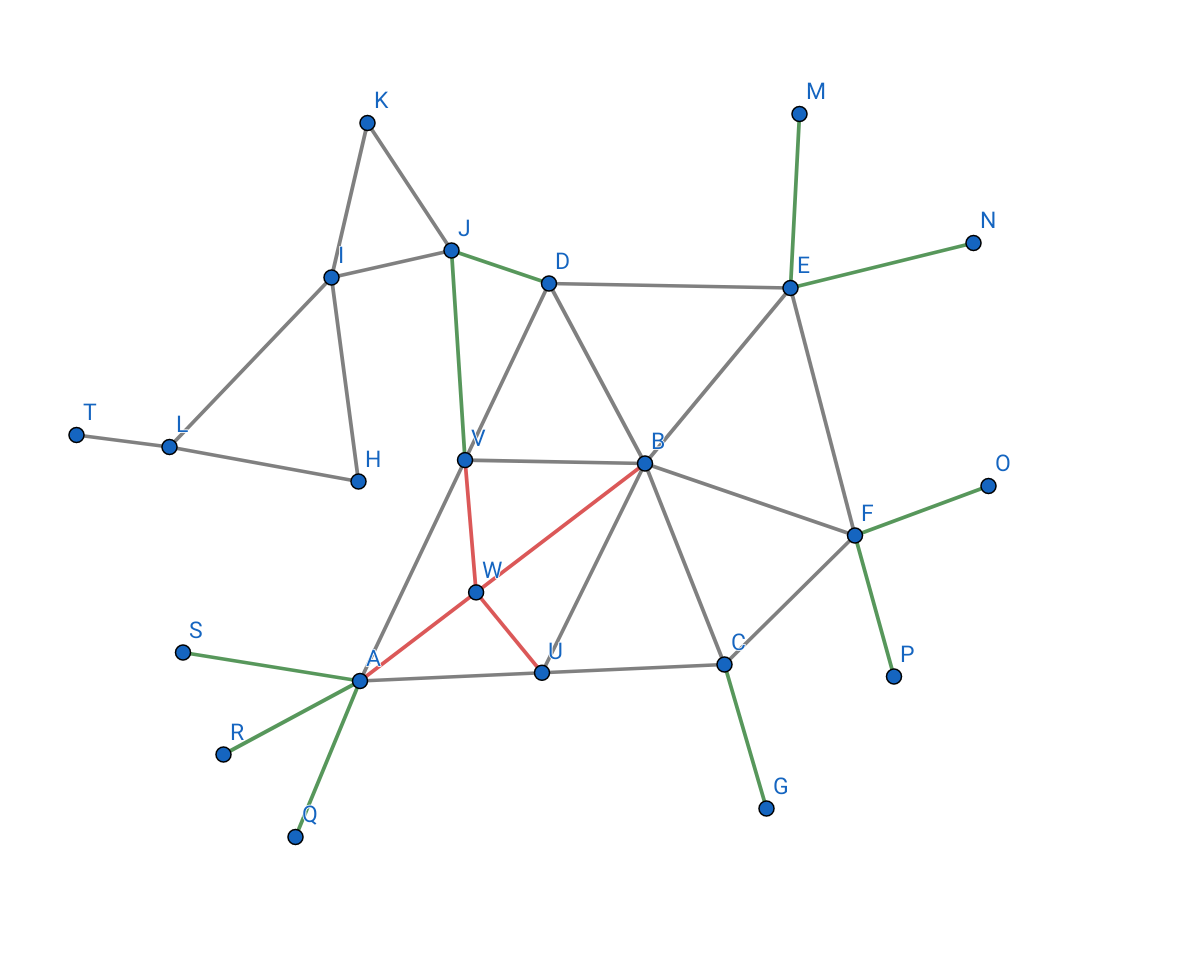
\includegraphics[scale = 0.3]{images/cobordo.jpg}
%\end{figure}

\begin{prop}
    The use of the coboundary operator makes sense only with antisimmetric functions on the edges, the antisimmetry of
    those function is somehow related to the orientation of surfaces.
\end{prop}
\begin{proof}
    $\sum_{\partial^0 \sum_{i \in \mc{A}} i}F_{ij} = \sum_{\sum_{i \in \mc{A}} \partial^0 i} F_{ij}$ if an edge
    is in the coboundary of two different vertexes of $\mc{A}$ it will be count twice, that means zero times in $\Z_2$,
    similarly for that same edge we would sum $F_{ij} + F_{ji} = 0$.
\end{proof}

    
\begin{defn}
    \underline{Graph laplacian}\\
    Let $f \in L^2(\mc{V})$ we have that $\scal{gradf}{gradf} = \scal{div(gradf)}{f} =: \scal{\Delta f}{f} = \scal{f}{\Delta f}$, where
    $\Delta : L^2(\mc{V}) \to L^2(\mc{V})$ is the Laplacian.
\end{defn}

\begin{prop}
    \underline{The laplacian represents the difference between the function and a local average of the function}\\
    (i) Graphs\\
    Let $w_{ii} = 0, and \sum_{j} w_{ij} = a_i$, i.e. normalized laplacian, we have that
    $(\Delta f)_i = f_i\frac{\sum_j w_{ij}}{a_i}-\sum_j\frac{w_{ij}}{a_i}f_j$ which is a weighted average.\\
    (ii) Manifolds (Let's just see it on an euclidean domain)\\
    Let $f_0 \int_{\partial B} dx - \int_{\partial B} dx f(x) \simeq \int_{\partial B} dx \scal{grad f}{x} = \int_B dx \Delta f$, where 
    B is a ball centered in 0 (or at least has a boundary), we have that $ f(0)-\frac{\int_{\partial B} dx f(x) f}{\int_{\partial B} dx}
    \simeq \frac{\int_B dx \Delta f}{\int_{\partial B} dx}$. Gauss theorem could be used since the incremental vector $x$ on a ball
    is parallel to $2x$ with is the gradient of the implicit function defining the ball.
    % La parte (ii) è molto brutta ma Francesco l'ha fatta bene
\end{prop}

%	Possibili approfondimenti interessanti:\\
%	(i)   Studio di equazioni differenziali sui grafi con gli operatori sopra definiti\\
%	      -Equazione del Calore\\
%	      $\frac{d(f_i)}{dt} = -c(\Delta f)_i$\\
%	      -Equazione di Schr$\ddot{o}$dinger\\
%	      $\frac{d(f_i)}{dt} = -c(\Delta f)_i + U_i f_i$\\
%	      -Equazione di Navier-Stokes\\
%	      -Equazione di continuità\\
%	      -altre\\
%	(ii)  Vincolare l'apprendimento di funzioni a divergenza nulla delle edge tramite $H^0$, eventuale applicazione a flussi incomprimibili\\
%	(iii) Definire il rotore per 2-simplessi e fare l'analogo con $H_1$, eventuale applicazione a reti elettriche tridimensionali\\
%       (iv)  Aggiungere la formalizzazione del cobordo e del bordo tramite gli operatori, ridefinizione della divergenza con il cobordo del vertice
%	(v)   Migliorare la formalizzazione dell'integrale sul percorso(da formalizzare come catena) ed il teorema del gradiente
%       (vi)  Coomologia di de Rahm per i grafi, bordo come aggiunto della derivata esterna
\end{document}
